\begin{tikzpicture}[
    declare function={
      gamma(\z)=(2.506628274631*sqrt(1/\z)+ 0.20888568*(1/\z)^(1.5)+ 0.00870357*(1/\z)^(2.5)- (174.2106599*(1/\z)^(3.5))/25920- (715.6423511*(1/\z)^(4.5))/1244160)*exp((-ln(1/\z)-1)*\z);},
    declare function={
      student(\x,\k) = (1/sqrt(3.14159265359*\k))*gamma((\k+1)/2)/gamma(\k/2)*(1+\x*\x/\k)^(-(\k+1)/2);}
]
\begin{axis}[
  width = 12cm, height = 6.5cm,
  xlabel = {$t$},
  ylabel = {Densité de probabilité},
  samples = 200,
  domain = -4.2:4.2,
  ymin = 0, ymax = 0.45,
  xtick = {-2.086, 0, 2.086},
  xticklabels = {$-t_{\nicefrac{\alpha}{2}}$, $0$, $t_{\nicefrac{\alpha}{2}}$},
  axis lines = left,
  clip = false,
  legend style = {draw=none, at={(0.02,0.98)}, anchor=north west}]

  % Les deux régions de rejet, de masse alpha/2 = 2,5 % chacune.
  \addplot[draw=none, fill=red!30, domain=-4.2:-2.086] {student(x,20)} \closedcycle;
  \addplot[draw=none, fill=red!30, domain=2.086:4.2]   {student(x,20)} \closedcycle;

  % La densité sous l'hypothèse nulle.
  \addplot[very thick, blue!70!black, mark={}] {student(x,20)};
  \addlegendentry{$t_{T-K}$ sous $\mathcal H_0$}

  % La statistique observée.
  \draw[very thick, red!80!black] (axis cs:2.9,0) -- (axis cs:2.9,0.30);
  \node[anchor=south, red!80!black, font=\footnotesize] at (axis cs:2.9,0.30)
       {$t^{\text{obs}}$};

  \node[anchor=south, red!70!black, font=\footnotesize] at (axis cs:-2.60,0.055)
       {$\nicefrac{\alpha}{2}$};
  \node[anchor=south, red!70!black, font=\footnotesize] at (axis cs:2.45,0.055)
       {$\nicefrac{\alpha}{2}$};
  \node[font=\footnotesize, align=center] at (axis cs:0,0.17)
       {Ne pas rejeter $\mathcal H_0$};
  \node[font=\footnotesize, red!70!black, align=center] at (axis cs:-3.35,0.14)
       {Rejeter};
  \node[font=\footnotesize, red!70!black, align=center] at (axis cs:3.35,0.14)
       {Rejeter};

\end{axis}
\end{tikzpicture}
